\documentclass[12pt,a4paper]{article}

\usepackage[american]{babel}
\usepackage{tocbibind}
\usepackage{parskip}
\usepackage[latin1]{inputenc}
\usepackage{a4wide}
\usepackage{makeidx}
\usepackage{url}
\usepackage{doc}
\usepackage{graphicx}
\usepackage{color}
\usepackage{amsmath}
\usepackage{amsfonts}
\usepackage{amssymb}
\usepackage{amsthm}
\usepackage{bbm}
\usepackage{enumerate}
\usepackage{bbold}

\makeatletter
\newcommand{\xout}[1]{%
  \ifmeasuring@
    % we're in the measuring stage, just use the argument
    #1
  \else
    % we're typesetting, add the strikeout rule
    \sbox0{$\displaystyle#1$}
    \rlap{\vrule height \dimexpr.5ex+0.4pt\relax
                 depth -\dimexpr.5ex-0.4pt\relax
                 width \wd0 }
    \box0
  \fi
}

\newcommand*{\centernot}{%
  \mathpalette\@centernot
}
\def\@centernot#1#2{%
  \mathrel{%
    \rlap{%
      \settowidth\dimen@{$\m@th#1{#2}$}%
      \kern.5\dimen@
      \settowidth\dimen@{$\m@th#1=$}%
      \kern-.5\dimen@
      $\m@th#1\not$%
    }%
    {#2}%
  }%
}
\makeatother

\numberwithin{equation}{section}

%%%%%%%%%%%%%%%%%%%%%%%%%%%%%%%%%%%%%%%%%%%%%%%%%%%%%%%%%%%%%%%%%%%%%%%%%%%%
% Sugar
%%%%%%%%%%%%%%%%%%%%%%%%%%%%%%%%%%%%%%%%%%%%%%%%%%%%%%%%%%%%%%%%%%%%%%%%%%%%

\newcommand{\independent}{\perp\mkern-9.5mu\perp}
\newcommand{\notindependent}{\centernot{\independent}}
\newcommand{\norm}[1]{\left\lVert#1\right\rVert}
\newcommand{\logit}[1]{\text{logit}\left(#1\right)}
\newcommand{\ilogit}[1]{\text{logit}^{-1}\left(#1\right)}
\newcommand{\expec}[2]{\mathbb{E}_{#1}\left[#2\right]}
\renewcommand{\P}{\mathbb{P}}
\renewcommand{\d}{\text{d}}
\newcommand{\simiid}{\stackrel{iid}{\sim}}
\newcommand{\trarrow}[1]{\xrightarrow{\text{#1}}}
\newcommand{\R}{\mathbb{R}}
\newcommand{\C}{\mathbb{C}}
\newcommand{\N}{\mathbb{N}}
\renewcommand{\O}{\mathcal{O}}
\newcommand{\Sp}{{\mathcal{S}_p}}
\newcommand{\ddx}[1]{\frac{\d}{\d #1}}
\newcommand{\Rp}{{\R^p}}
\newcommand{\F}{\mathcal{F}}
\renewcommand{\Finv}{{\mathcal{F}^{-1}}}
\newcommand{\abs}[1]{\left|#1\right|}
\newcommand{\intRp}[2]{\int_{\Rp} #2 \d #1}
\newcommand{\expf}[1]{\exp\left(#1\right)}
\newcommand{\expfc}[1]{\exp\left\{#1\right\}}
\newcommand{\logf}[1]{\log\left(#1\right)}

%%%%%%%%%%%%%%%%%%%%%%%%%%%%%%%%%%%%%%%%%%%%%%%%%%%%%%%%%%%%%%%%%%%%%%%%%%%%
% Theorems setup
%%%%%%%%%%%%%%%%%%%%%%%%%%%%%%%%%%%%%%%%%%%%%%%%%%%%%%%%%%%%%%%%%%%%%%%%%%%%
\newtheoremstyle{def}
  {12pt}   % ABOVESPACE
  {6pt}   % BELOWSPACE
  {\normalfont}  % BODYFONT
  {0pt}       % INDENT (empty value is the same as 0pt)
  {\bfseries} % HEADFONT
  {.}         % HEADPUNCT
  {5pt plus 1pt minus 1pt} % HEADSPACE
  {}          % CUSTOM-HEAD-SPEC

\theoremstyle{def}
\newtheorem{theorem}{Theorem}[section]
\theoremstyle{def}
\newtheorem{lemma}[theorem]{Lemma}
\theoremstyle{def}
\newtheorem{corollary}[theorem]{Corollary}
\theoremstyle{def}
\newtheorem{example}[theorem]{Example}
\theoremstyle{def}
\newtheorem{assumption}[theorem]{Assumption}
\newtheorem*{remark}{Remark}
\newtheorem*{remarks}{Remarks}
\theoremstyle{def}
\newtheorem{definition}[theorem]{Definition}

\graphicspath{{figures/}}

\global\newcommand{\note}[1]{{\color{red}(#1)}}

\title{Higher-order statistics got high-dimensional problems with applications to graphical models}
\author{Matthieu Bult\'e}

\begin{document}

% \maketitle
% \newpage

% \begin{itemize}
    \item {
        2020-10-??: Section 6.2 (p174, $p^*$-formula of \cite{BarndorffNielsen1994}, jumping back to 
        \begin{itemize}
            \item 2.5 (p36): Ancilliarity
            \item {5.2 (p145): Log-likelihood derivatives and mixed log model derivatives.\\
                Barlett Identities, balance relations
            }
            \item 5.4 (p155): {Expansion of likelihood quantities: observed case\\
                More expansions based on results in 5.2
            }
        \end{itemize}
    }
    \item {
        2020-12-02:
        \begin{itemize}
            \item The $p^*$ formula and other approximation formula provide an approximation for the distribution of the MLE $\hat\theta$.
            \item Using this approximation, one can compute an approximation to the density of other statistics by change of variable formula: this is true because with $A$ ancilliary, $(\hat\theta, A)$ is sufficient (always?).
            \item The above point also works for components of the MLE (profile likelihood setting) where the variable of interest is $\psi$ in $\theta = (\psi, \chi)$. See the derivation for $r^*$ in \cite[Section 6.6.1]{BarndorffNielsen1994}.
            \item So to understand this whole story, need to understand the multi variate version of the $p^*$ formula $\rightarrow$ multi variate version of the saddlepoint approximation.
            \item Still not sure about the whole Ancilliarity topic and how it is applied.
        \end{itemize}
    }
    \item{
        2020-12-08:
        \begin{itemize}
            \item The whole point of all of this is to estimate (with some series expansion) the distribution of a certain quantity, say $r^\star$.
            \item Since we know that some of them converge to a known distribution ($N(\mu, \sigma^2) ,\chi^2_p$), we want to factorize the approximate density as $f_{\text{known distribution}} \times (1 + \mathcal{O}(n^{-\varphi}))$
        \end{itemize}
    }
\end{itemize}


\begin{align*}
    \left| \hat\theta_{/(r, \hat\lambda_{\psi_0})} \right|
    &= \left| \left(\ell_{;\hat\theta}(\hat\theta; \hat\theta) - \ell_{;\hat\theta}(\hat\theta_{\psi_0}; \hat\theta); \ \ \ell_{\lambda; \hat\theta}(\hat\theta_{\psi_0}; \hat\theta) \right) \right|^{-1} \left| \left(\begin{matrix}
        r & 0\\
        0 & j_{\lambda\lambda}(\hat\theta_{\psi_0})
    \end{matrix}\right) \right|\\
    &= r \left| j_{\lambda\lambda}(\hat\theta_{\psi_0}) \right| \left| \left(\ell_{;\hat\theta}(\hat\theta; \hat\theta) - \ell_{;\hat\theta}(\hat\theta_{\psi_0}; \hat\theta); \ \ \ell_{\lambda; \hat\theta}(\hat\theta_{\psi_0}; \hat\theta) \right) \right|^{-1},
\end{align*}
and hence
\begin{equation*}
    \left| (r, \hat\lambda_{\psi_0})_{/\hat\theta}\right| = \left| \hat\theta_{/(r, \hat\lambda_{\psi_0})} \right|^{-1} = r^{-1} \left| j_{\lambda\lambda}(\hat\theta_{\psi_0}) \right|^{-1} \left| \left(\ell_{;\hat\theta}(\hat\theta; \hat\theta) - \ell_{;\hat\theta}(\hat\theta_{\psi_0}; \hat\theta); \ \ \ell_{\lambda; \hat\theta}(\hat\theta_{\psi_0}; \hat\theta) \right) \right|
\end{equation*}


% \section{Summary}

\subsection{Introduction}

Assume a parametric model for i.i.d.\ observations $(Y_1, \ldots, Y_n)$ where $Y_i \sim F(\theta)$, the distribution $F(\theta)$ has a density $f(\cdot; \theta)$ and $\theta \in \mathbb{R}^p$. We only wish to perform inference on a one-dimensional parameter $\psi$, leading to the decomposition $\theta = (\psi, \lambda)$ with $\lambda \in \mathbb{R}^{p-1}$. The parameters $\psi$ and $\lambda$ are also referred to as \textit{parameter of interest} and \textit{nuisance parameters}. This is the same setting used in Tang et al. \cite{Tang2020}.

To simplify the discussion, we will (at least for now) assume that $F(\theta)$ is a member of an $(m,m)-$exponential family with natural parameter $\theta$. Hence, we know that the MLE $\hat\theta$ is sufficient\footnote{In a more general setting, one would need to consider an additional statistic $a$ which is either approximately or exactly ancilliary for $(\hat\theta, a)$ to be used as a sufficient statistic.} and can replace the conditionning of the likelihood on the data with a conditionning on $\hat\theta$ and write $\ell(\theta; y) = \ell(\theta; \hat\theta)$. 

We define the \textit{profile log-likelihod} $\ell_p$ and \textit{normalized profile log-likelihood} $\bar\ell_p(\psi)$,
\begin{align*}
    \ell_p(\psi) = \sup_{\lambda} \ell(\psi, \lambda) && \text{and} && \bar\ell_p(\psi) = \ell_p(\hat\psi) - \ell_p(\psi).
\end{align*}
Under the model $F(\theta)$ with $\psi = \psi_0$, the the \textit{directed likelihood root} is 
\begin{equation*}
    r(\psi_0) = \text{sgn}(\hat\psi - \psi_0)\left[2 \bar\ell_p(\psi_0)\right]^{1/2}.
\end{equation*}
For fixed $p$ and under regularity conditions, the directed profile likelihood converges to a $N(0, 1)$ random variable with relative error of $O(n^{-1/2})$. This convergence will be explored in following sections. A modified version can be more accurately approximated by the standard normal, the \textit{modified likelihood root}, given by
\begin{equation}
    r^\star(\psi_0) = r(\psi_0) + r(\psi_0)^{-1}\log\left[C(\psi_0)\tilde u(\psi_0) / r(\psi_0)\right],
\end{equation}
with
\begin{align*}
    \tilde u(\psi_0) = j_p^{-1/2}(\hat\psi)\bar\ell_{p/\hat\psi}(\psi_0) && \text{and} && C(\psi_0) = |\ell_{\lambda; \hat\lambda}(\hat\theta_{\psi_0})| / \{ |j_{\lambda\lambda}(\hat\theta_{\psi_0})||j_{\lambda\lambda}(\hat\theta)| \}^{1/2}
\end{align*}

Under the same regularity conditions, the normal distribution approximates the distribution of $r^\star$ with relative error of $O(n^{-3/2})$.

\subsection{Approximation to the distribution of $\hat\theta$}

As we will show in the next Section, the distribution of both $r$ and $r^\star$ can be expressed via a change of variable s proportional to the distribution of the MLE $\hat\theta$. Hence, finding   asymptoticaly valid approximations to the distribution of $\hat\theta$ will be used to derive similar approximations to the distribution of $r$ and $r^\star$.

Continuing with the setup of the previous section, we assume that we have access to a sample of $n$ i.i.. observations $(Y_1, \ldots, Y_n)$ from an exponential family $F(\theta)$. Since $F(\theta)$ is an exponential family, we can assume that its density has the form
\begin{equation*}
    f_Y(y; \theta) = \exp\left(\theta^\top y - \mathcal{H}_Y(\theta) - \mathcal{G}_Y(y)\right)
\end{equation*}
and the cumulant generating function of $Y$ is given by
\begin{equation*}
    \mathcal{K}_Y(\beta; \theta) = \mathcal{H}_Y(\theta + \beta) - \mathcal{H}_Y(\theta).
\end{equation*}

Assume that $Y$ is centered\footnote{This is to simplify the notation. It will be removed in the future}, that is, $\mathbb{E}_\theta[Y] = 0$ and let $S_n$ be the standardized mean of $Y_1, \ldots, Y_n$. We can construct a Saddlepoint approxmiation\footnote{Details on the Saddlepoint approximation will come in the future.} to the distribution of $S_n$, giving
\begin{equation} \label{eq-saddlepoint-sn}
    f_{S_n}(s; \theta) = \frac{\exp\left(n\left[\mathcal{K}_Y(\hat\beta; \theta) - \hat\beta^\top s\right]\right)}{\left| \mathcal{K}^{''}_Y(\hat\beta; \theta) \right|^{1/2}}\left(\frac{n}{2\pi}\right)^{p/2}\left[ 1 + \frac{b(\hat\beta)}{2n} + O(n^{-2}) \right],
\end{equation}
where $\hat\beta$ solves $\mathcal{K}^{'}_{Y}(\hat\beta; \theta) = s$. Since the $Y_i$ are from an exponential family, its cumulant generating function has the special form $\mathcal{K}_Y(\beta; \theta) = \mathcal{H}_Y(\theta + \beta) - \mathcal{H}_Y(\theta)$ and hence the condition on $\hat\beta$ is equivalent to $\mathcal{H}^{'}_{Y}(\theta + \hat\beta) = s$. Furthermore, using again the properties of exponential families, we have that the MLE $\hat\theta$ satisfies $\mathcal{H}^{'}_{Y}(\hat\theta) = s$ and hence $\hat\beta = \hat\theta - \theta$. Replacing this in (\ref{eq-saddlepoint-sn}) together with some rewriting yields
\begin{equation} \label{eq-saddlepoint-nobeta}
    f_{S_n}(s; \theta) = \frac{\exp\left( \ell(\hat\theta) - \ell(\theta) \right)}{\left| j(\hat\theta) \right|^{1/2}\left(2\pi\right)^{p/2}}\left[ 1 + \frac{b(\hat\beta)}{2n} + O(n^{-2}) \right].
\end{equation}

Finally, we note that since $\mathcal{H}^{'}_{S_n}(\hat\theta) = s$ and $\frac{\d}{\d s}\mathcal{H}^{'}_{S_n} = \hat\theta_{/s}\mathcal{H}^{''}_{S_n}(\hat\theta)$, we get that $\hat\theta_{/s} = \mathcal{H}^{''}_{S_n}(\hat\theta)^{-1} = j(\hat\theta)^{-1}$ and hence by change of varible we can obtain an approximation to the density of $\hat\theta$ 
\begin{equation*} \label{eq-unnormalized-pstar}
    f_{\hat\theta}(\hat\theta; \theta) = \left(2\pi\right)^{-p/2}\left| j(\theta) \right|^{1/2}  \exp\left( \ell(\hat\theta) - \ell(\theta) \right) \left[ 1 + \frac{b(\hat\beta)}{n} + O(n^{-2}) \right].
\end{equation*}

Note that Approximation (\ref{eq-unnormalized-pstar}) need not integrate to 1. Dividing the approximation by a factor of $1 + \frac{b(0)}{2n}$ can be shown to yield an approximation of order $O(n^{-3/2})$ which is also a proper density function. The resulting approximation is a special case of the \textit{Barndorff-Nielsen formula} also called $p^\star$ \textit{formula}.

\subsection{Distribution of $r^\star$}

High-order approximations to the distribution of the MLE $\hat\theta$ can be readily found as we will show in later sections. By change of variable, such approximations can be used to derive approximnations to the distribution of both the directed and modified likelihood roots $r$ and $r^\star$. We follow the derivation presented in Barndorff-Nielsen and Cox \cite{BarndorffNielsen1994}.

First, we assume that such a change of variable exists between the MLE $\hat\theta = (\hat\psi, \hat\lambda)$ and a vector composed of the directed likelihood root and the profile MLE $\hat\lambda_{\psi_0}$. To determine the Jacobian of this transformation, we consider the equations determining $r$ and $\hat\lambda_{\psi_0}$,
\begin{align*}
    \ell(\hat\theta; \hat\theta) - \ell(\hat\theta_{\psi_0}; \hat\theta) &= \frac12r^2\\
    \ell_\lambda(\hat\theta_{\psi_0}; \hat\theta) &= 0.
\end{align*}
Taking derivatives of these two equations with respect to $r$ and $\hat\lambda_{\psi_0}$, while keeping the other fix, yields the following additional equations
\begin{align}
    \hat\theta_{/r} \left\{ \ell_{;\hat\theta}(\hat\theta; \hat\theta) - \ell_{;\hat\theta}(\hat\theta_{\psi_0}; \hat\theta) \right\} &= r \label{A}\\
    \hat\theta_{/\hat\lambda_{\psi_0}} \left\{ \ell_{;\hat\theta}(\hat\theta; \hat\theta) - \ell_{;\hat\theta}(\hat\theta_{\psi_0}; \hat\theta) \right\} &= 0\\
    \hat\theta_{/r}\ell_{\lambda; \hat\theta}(\hat\theta_{\psi_0}; \hat\theta) &= 0\\
    \ell_{\lambda\lambda}(\hat\theta_{\psi_0}; \hat\theta) + \hat\theta_{/\hat\lambda_{\psi_0}}\ell_{\lambda; \hat\theta}(\hat\theta_{\psi_0}; \hat\theta) &= 0. \label{eq-score-4}
\end{align}

We first note that $\ell_{\lambda\lambda}(\hat\theta_{\psi_0}; \hat\theta) = -j_{\lambda\lambda}(\hat\theta_{\psi_0})$, which implies together with (\ref{eq-score-4}) that $\hat\theta_{/\hat\lambda_{\psi_0}}\ell_{\lambda; \hat\theta}(\hat\theta_{\psi_0}; \hat\theta) = j_{\lambda\lambda}(\hat\theta_{\psi_0})$. All together we have
\begin{equation*}
    \hat\theta_{/(r, \hat\lambda_{\psi_0})} \left(\ell_{;\hat\theta}(\hat\theta; \hat\theta) - \ell_{;\hat\theta}(\hat\theta_{\psi_0}; \hat\theta); \ \ \ell_{\lambda; \hat\theta}(\hat\theta_{\psi_0}; \hat\theta) \right) = 
    \left(\begin{matrix}
        r & 0\\
        0 & j_{\lambda\lambda}(\hat\theta_{\psi_0})
    \end{matrix}\right),
\end{equation*}
which after a some rewriting yields,
\begin{equation*}
    \left| \hat\theta_{/(r, \hat\lambda_{\psi_0})} \right| 
    = r \frac{\left| j_{\lambda\lambda}(\hat\theta_{\psi_0}) \right|}{\bar\ell_{p/\hat\psi}(\psi_0)\left| \ell_{\lambda;\hat\lambda}(\hat\theta_{\psi_0}) \right|}.
\end{equation*}



% \newpage

\subsection{Charlier differential Series}

Let $F, G$ be two distributions with characteristic functions $\chi, \xi$ and cumulants $\beta_r, \gamma_r$ for $r \geq 1$. We assume that the derivatives $F^{(r)}(x), G^{(r)}(x)$ exist for all $r \geq 1$ and vanish when $x$ approaches the boundaries of the domain of definition \note{this is handwavy}. We first note the following relation
\
\begin{align*}
    \beta_r
    &= \frac{\d^r}{\d u^r} K_F(u) |_{u=0}
    = \frac{\d^r}{\d u^r} \log \mathbb{E}_F\left[\exp(uX)\right]|_{u=0}\\
    &= \frac{\d^r}{\d u^r} \log \mathbb{E}_F\left[\exp(uX)\right]|_{u=0}
    = i^{-r}\frac{\d^r}{\d u^r} \log \mathbb{E}_F\left[\exp(iuX)\right]|_{u=0}\\
    &= (-i)^r\frac{\d^r}{\d u^r} \log \chi(u) |_{u=0}
\end{align*}
\
By Taylor expansion of $\log \chi(u)$ around $u = 0$ and using that $\chi(0) = 1$, we obtain
\begin{equation*}
    \log \chi(u)
    = \log \chi(0) + \sum_{r=1}^\infty \frac{u^r}{r!}\frac{\d^r}{\d u^r} \log \chi(u) |_{u=0}
    = \sum_{r=1}^\infty \frac{(iu)^r}{r!}\beta_r.
\end{equation*}
\
This result holds accordingly for $\xi$, giving
\begin{align*}
    \log \frac{\chi(u)}{\xi(u)} &= \sum_{r=1}^\infty (\beta_r - \gamma_r)\frac{(iu)^r}{r!}\\
\Rightarrow \chi(u) &= \xi(u) \exp\left\{\sum_{r=1}^\infty (\beta_r - \gamma_r)\frac{(iu)^r}{r!}\right\}.
\end{align*}
\
\note{properly introduce the fourier transform somewhere else, since we use the "stats" version of fourier which is different from the usual $L^2$ operator}

We can now show that $u \mapsto (iu)^r\xi(u)$ is the characteristic function of $x \mapsto (-1)^rG^{(r)}(x)$, or $(iu)^r\xi(u) = \mathcal{F}\left[(-1)^rG^{(r+1)}\right](u)$, since by integration by part we have
\begin{align*}
    \mathcal{F}\left[(-1)^rG^{(r+1)}\right](u)
    &= \int_{\mathbb{R}} e^{iux}(-1)^rG^{(r+1)}(x) dx \\
    &= \left[e^{iux}(-1)^rG^{(r)}(x)\right]_{-\infty}^{+\infty} - \int_{\mathbb{R}} (iu)e^{iux}(-1)^rG^{(r)}(x)dx\\
    &= iu \int_{\mathbb{R}} e^{iux}(-1)^{r-1}G^{(r)}(x) dx
    = (iu)\mathcal{F}\left[(-1)^{r-1}G^{(r)}\right](u)\\
    &= \ldots = (iu)^r\mathcal{F}\left[G^{(1)}\right] = (iu)^r \xi(u).
\end{align*}

With $\alpha_r = \beta_r - \gamma_r$ and vy Taylor expansion, we can rewrite
\begin{align*}
    \chi(u)
    &= \xi(u)\exp\left\{\sum_{r=1}^\infty \alpha_r\frac{(iu)^r}{r!}\right\} \\
    &= \xi(u)\sum_{l=0}^\infty \frac{1}{l!}\left\{\sum_{r=1}^\infty \alpha_r\frac{(iu)^r}{r!}\right\}^l \\
    &= \sum_{l=0}^\infty \frac{1}{l!} \sum_{r_1, \ldots, r_l=1}^\infty \alpha_{r_1}\ldots\alpha_{r_l}\frac{\xi(u)(iu)^{r_1 + \ldots + r_l}}{r_1!\ldots r_l!}
\end{align*}
And hence, by linearity of the inverse Fourier transform, \note{very handwavy}
\begin{align*}
    F^{(1)} = \mathcal{F}^{-1}\left[\chi\right]
    &= \sum_{l=0}^\infty \frac{1}{l!} \sum_{r_1, \ldots, r_l=1}^\infty \alpha_{r_1}\ldots\alpha_{r_l}\frac{\mathcal{F}^{-1}\left[\xi(u)(iu)^{r_1 + \ldots + r_l}\right]}{r_1!\ldots r_l!}\\
    &= \sum_{l=0}^\infty \frac{1}{l!} \sum_{r_1, \ldots, r_l=1}^\infty \alpha_{r_1}\ldots\alpha_{r_l}\frac{(-1)^{r_1 + \ldots + r_l}G^{(r_1 + \ldots + r_l + 1)}}{r_1!\ldots r_l!}\\
    &= \sum_{l=0}^\infty \frac{1}{l!} \sum_{r_1, \ldots, r_l=1}^\infty \alpha_{r_1}\ldots\alpha_{r_l}\frac{(-D)^{r_1 + \ldots + r_l}G^{(1)}}{r_1!\ldots r_l!}\\
    &= \exp\left\{\sum_{r=1}^\infty \alpha_r\frac{(-D)^r}{r!}\right\}G^{(1)},
\end{align*}
where $D$ is the differential operator with respect to $x$ and $\exp D = \sum_{l=0}^\infty \frac{D^l}{l!}$. All in all, we obtain an expansion for the density $f = F^{(1)}$ of $F$ in terms of $G$ and the cumulants of both distributions,
\begin{equation}\label{eq-charlier}
    f(x) = \exp\left\{\sum_{r=1}^\infty (\beta_r - \gamma_r)\frac{(-D)^r}{r!}\right\}g(x).
\end{equation}
Using $G = \Phi$, where $\Phi$ is the distribution function of $N(0, 1)$, in expansion (\ref{eq-charlier}) is called a Charlier differential series.
\newpage

\section{Notation}

\paragraph{Indexing} Multi-indexable objects are indexed by writing indices in the exponent of the variables. For instance, we use $A^{ij}$ to denote the element in the $i$-th row of the $j$-th column of a matrix $A \in \mathbb{R}^{n\times m}$.

\paragraph{Einstein notation} A term given in the Einstein notation can be rewritten as a correct turn by remplacing any free index on a vector or matrix quantity by a sum of the indexed quantity over the range of meaningful possible values. For instance, let $v, w \in \mathbb{R}^n$, we can write
\begin{equation*}
    v^iw^i = \sum_{i=1}^n v^iw^i. 
\end{equation*}


\paragraph{Partial derivatives} For $R = (r_1, \ldots, r_n)$ and $S = (s_1, \ldots, s_m)$
\begin{equation*}
    \ell_{R;S}(\theta_0) = \left[\frac{\partial^{n+m}\ell(\theta; \hat\theta, a)}{\partial\theta^{r_1} \ldots \partial\theta^{r_n}\partial\hat\theta^{s_1} \ldots \partial\hat\theta^{s_m}}\right]_{\theta=\theta_0}.
\end{equation*}


\section{Definitions}

\begin{definition}
    An anciliary statistic of a statistical model $p(x; \theta)$ is a pivotal statistic, that is, a function of the sample of which the distribution does not depend on the parameter $\theta$ of the model.
\end{definition}

\begin{example} \label{ex-normal}
    Let $X_1, \ldots, X_n \simiid N(\theta, 1)$, the sample variance,
    \begin{equation*}
        \hat\sigma^2 = \frac{\sum_{i=1}^n (X_i - \bar X)^2}{n},
    \end{equation*}
    is an anciliary statistic.
\end{example}

\begin{example} \label{ex-loc-model}
    Let $Y_1, \ldots, Y_n \simiid h(\cdot - \mu)$ follow a location model with location parameter $\mu$. The \textit{orbit}, $a = (Y_{(2)} - Y_{(1)}, \ldots, Y_{(n)} - Y_{(1)})$ is an anciliary statistic since $a$ is invariant under translation. Since the transformation $y_{(1)} \rightarrow y_{(1)}, y_{(2)} \rightarrow y_{(1)} + a_1, \ldots, y_{(n)} \rightarrow y_{(1)} + a_{n-1}$ has unit Jacobian, we get that the joint density of $(Y_{(1)}, A)$ is
    \begin{equation*}
        n!h(y_{(n)} - \mu)h(y_{(n)} + a_1 - \mu)\ldots h(y_{(n)} + a_{n-1} - \mu)
    \end{equation*}
    And the density of $Y_{(1)}$ given $A = a$ is given by
    \begin{align*}
        p(y_{(1)} | a; \mu) &= \frac{h(y_{(n)} - \mu)h(y_{(n)} + a_1 - \mu)\ldots h(y_{(n)} + a_{n-1} - \mu)}{\int{h(z - \mu)h(z + a_1 - \mu)\ldots h(z + a_{n-1} - \mu)}\d z}\\
        &= \frac{\ell(\mu; u)}{\int{L(\nu; y) \d \nu}}.
    \end{align*}
    This shows that the conditional distribution of the position parameter $Y_{(1)}$ is equal to the normalized likelihood of $\mu$. Note that for $a$ fix, the right hand side is then a function of the difference $y_{(1)} - \mu$.
\end{example}

\begin{definition}
    Given a model with parameters $\theta = (\psi, \lambda)$ where $\psi$ is the paramter of interest and $\lambda$ is a vector of nuisance parameters, we define the profile likelihood as
    \begin{equation*}
        L_P(\psi; x) = \max_{\lambda} L(\psi, \lambda; x) \equiv L(\psi, \lambda_\psi; x).
    \end{equation*}
\end{definition}
\begin{example}
    Consider the linear regression model $Y \sim N(X\beta, \tau 1_n)$ where $Y$ is a vector of $n$ observations and $\beta$ is a vector of $d_\beta < n$ parameters. The parameter of interest is the error variance $\tau$. Then the MLE of $\tau$ is $\hat\tau = SSD / n$ has a expected value of $\tau (n - d_\beta)/n$ and hence a bias of $-\tau d_\beta/n$. This means that if $d_\beta = d_{\beta(n)}$ is allowed to vary with $n$, in particular if $d_{\beta(n)} = O(n)$, the MLE for $\tau$ is biased.
\end{example}

\begin{definition}
    A conditionality resolution of a statistical model $p(x; \theta)$ is a one-to-one transformation of the minimal sufficient statistic $t$ to the statistic $(\hat\theta, a)$, where $\hat\theta$ is the MLE of $\theta$ and $a$ is an anciliary statistic, and $p(\hat\theta; \theta | a)$ has a \textit{manageable} expression.
\end{definition}

\begin{example}
    In the normal model of Example \ref{ex-normal}, it can be easily shown that $t = (\bar x, \hat\sigma^2)$ is minimal sufficient. Taking the lof of the model function can then be rewritten as
    \begin{equation*}
        p(x; \theta) = - n\hat\sigma^2 - n(\bar x - \theta)^2.
    \end{equation*}
    Since $\hat\theta = \bar x$ and $\hat\sigma^2$ is anciliary, we can say that the minimal sufficient statistic $t$ is itself a conditionality resolution.
    \note{maybe not a great example}
\end{example}

\begin{definition}
    A curved exponential model, or $(m, d)$ exponential model, $\{ P_\theta : \theta \in \mathbb{R}^d \}$ is a model with model function
    \begin{equation*}
        p(x; \theta) = a(\phi(\theta))b(x)e^{\langle s(x), \phi(\theta)\rangle},
    \end{equation*}
    where $s(x)$ and $\phi(\theta)$ are of dimension $m > d$.
\end{definition}

\begin{remark}
    The following holds,
    \begin{itemize}
        \item $\eta(\theta) := \mathbb{E}_\theta[s(X)]$;
        \item $\frac{\partial}{\partial \phi_i} \log a(\phi) = -\eta_i$
        \item $\ell = \log a(\phi) + s^i(x)\phi^i$
        \item $\ell_r = \phi^i_r(s^i - \eta^i)$
        \item $\hat\phi^\top_r(s - \hat\eta) = 0 \Rightarrow \hat\phi_r \perp s - \hat\eta$
    \end{itemize}
\end{remark}





\subsection{Observed information}

Given that our model of interest has a conditionality resolution, we can also express the log-likelihood via $(\hat\theta, a)$ as $\ell(\theta; \hat\theta, a)$. We then use the follwoing notation: $\ell = \ell(\theta; \hat\theta, a)$, $\hat\ell = \ell(\hat\theta; \hat\theta, a)$ and $\xout\ell = \ell(\theta; \theta, a)$. Quantities like $\hat\ell_{R;S}$ or $\xout\ell_{R;S}$ are taken by substituting $\theta$ or $\hat\theta$ after all differentiations have taken place.

The observed information is given by $j_{rs} = -\ell_{rs}$. We can extend the $\hat\ell$ and $\xout\ell$ notation to $j$ to define $\hat j$ and $\xout j$.


\begin{definition}
    Normed log-likelihood $\bar\ell$ as 
    \begin{equation*}
        \bar\ell(\theta; \hat\theta, a) = \ell(\theta; \hat\theta, a) - \ell(\hat\theta; \hat\theta, a).
    \end{equation*}
        
\end{definition}


\begin{definition}
    The $p^\star$-formula is defined by
    \begin{equation}\label{def-pstar}
        p^\star(\hat\theta; \theta | a) = c |\hat j|^{1/2}e^{\bar \ell},
    \end{equation}
    where $a$ is anciliary and $c = c(\theta, a)$ is a normalizing constant such that $p^\star$ integrated over the range of possible values of $\hat\theta$ is unity.
\end{definition}




\begin{definition}
    Gaussian Graphical Model.
    \begin{equation*}
        p(x; \Theta) = \frac{|\Theta|^{1/2}}{(2\pi)^{m/2}} \exp\left( -\frac12x^\top\Theta x \right)
    \end{equation*}
\end{definition}

% \section{Gaussian Graphical Models}

\subsection{Notation}
Let $\mathcal{S}_p$ be the set of symmetric positive definite $p \times p$ matrices. We define the vector representation of a symmetric positive definite matrix by the mapping $\text{vec} : \mathcal{S}_p \rightarrow \mathbb{R}^{p(p+1)/2}$ given by
\begin{equation*}
    \text{vec}(A) = \text{vec}\left(\begin{matrix}
        a_{1,1} & a_{2, 1} & \ldots & a_{p, 1} \\
        a_{2,1} & a_{2, 2} & \ldots & a_{p, 2} \\
                &          & \ldots & \\
        a_{p,1} & a_{p, 2} & \ldots & a_{p, p}
    \end{matrix}\right) = \left( a_{1,1}, a_{2,1}, a_{2,2}, \ldots, a_{p, p} \right)^\top, \ \forall A \in \mathcal{S}_p.
\end{equation*}

We define $\text{vec}(\mathcal{S}_p)$ to be the image of $\mathcal{S}_p$ under vec and $\text{mat} : \text{vec}(\mathcal{S}_p) \rightarrow \mathcal{S}_p$ be the inverse mapping of vec.

% Let $A \in \mathbb{R}^{p \times p}$ and $\mathcal{C} \subset \{1, \ldots, p \}$, then we define $A^{(\mathcal{C})} \in \mathbb{R}^{|\mathcal{C}| \times |\mathcal{C}|}$ as
% \begin{equation*}
%     A^{(\mathcal{C})}_{ij} = a
% \end{equation*}

\subsection{Definition}
Let $X$ be a random vector of dimension $p$ distributed according to the centered \textit{multivariate Gaussian} distribution $\mathcal{N}_p(0, \Sigma)$, where $\Sigma \in \mathcal{S}_p$ is called the \textit{covariance matrix}. The multivariate normal distribution has density function
\begin{equation*}
    f(x; \Sigma) = (2\pi)^{-p/2} |\Sigma|^{-1/2} \exp\left(-\frac{1}{2} x^\top\Sigma^{-1}x\right).
\end{equation*}
We define the \textit{precision matrix} $\Omega \in \mathcal{S}_p$ as the inverse of the covariance matrix, $\Omega = \Sigma^{-1}$. Furthermore, since $x^\top\Sigma^{-1} x \in \mathbb{R}$ and using the cyclic property of the trace, we have that $x^\top\Sigma^{-1} x = \text{tr}\left(x^\top\Sigma^{-1} x\right) = \text{tr}\left(xx^\top\Sigma^{-1}\right)$. This allows the following characterization of the density function of the multivariate normal distribution
\begin{equation} \label{eq-density-omega}
    f(x; \Omega) = (2\pi)^{-p/2} |\Omega|^{1/2} \exp\left(-\frac{1}{2} \text{tr}\left(xx^\top\Omega\right)\right),
\end{equation}

Given a random sample $X^{(1)}, \ldots, X^{(n)} \simiid \mathcal{N}_p(0, \Omega^{-1})$ we define the data matrix $X = (X^{(1)}, \ldots, X^{(n)})$, giving the log-likelihood function
\begin{equation} \label{eq-ll-omega}
    \ell(\Omega; X) = -\frac{np}{2}\log(2\pi) + \frac{n}{2}\log |\Omega| - \frac{1}{2} \text{tr}\left(XX^\top\Omega\right).
\end{equation}
For convenience, we will sometimes directly write $\ell(\Omega)$ to mean $\ell(\Omega; X)$.

\subsection{Maximum likelihood estimator of the precision matrix}

We are now interested in finding the maximum likelihood estimator of the precision matrix. To do so, we look for solutions $\hat\Omega$ to the score equation $\frac{\d}{\d\Omega}\ell(\Omega)|_{\Omega=\hat\Omega} = 0$. Using that $\frac{\partial}{\partial A_{ij}} \log|A| = A_{ij}^{-\top}$ and $\frac{\partial}{\partial A_{ij}} \text{tr}(B A) = B_{ij}^\top$ for any $A, B \in \mathbb{R}^{p \times p}$ and $i, j = 1, \ldots, p$, we can compute partial derivatives of the log-likelihood
\begin{equation*}
    \frac{\partial}{\partial\Omega_{ij}}\ell(\Omega) 
    = \frac{n}{2}\left(\Omega^{-\top}\right)_{ij} - \frac{1}{2}\left(XX^\top\right)_{ij}^\top
    = \frac{n}{2}\left(\Omega^{-1}\right)_{ij} - \frac{1}{2}\left(XX^\top\right)_{ij},
\end{equation*}
We first consider the model in which no assumptions are made on the independence relations of the components of each random vector $X^{(k)}$. In this case, the maximum likelihood estimator $\hat\Omega$ must satisfy $\frac{\partial}{\partial\Omega_{ij}}\ell(\hat\Omega) = 0$ for all $i, j = 1, \ldots, p$. Assuming that $XX^\top$ is invertible and combining the score equations yields
\begin{equation*}
    \frac{n}{2}\hat\Omega^{-1} - \frac{1}{2}XX^\top = 0 \Rightarrow \hat\Omega = \left(\frac{1}{n}XX^\top\right)^{-1}.
\end{equation*}

Note that this shows that the unconstrained maximum likelihood estimator $\hat\Omega$ is a sufficient statistic, and we can re-express the log-likelihood $\ell(\Omega; X)$ in terms of $\hat\Omega$ instead of $X$ as
\begin{equation}\label{eq-ll-mle}
    \ell(\Omega; \hat\Omega) = -\frac{np}{2}\log(2\pi) + \frac{n}{2}\log |\Omega| - \frac{n}{2} \text{tr}\left(\hat\Omega^{-1}\Omega\right),
\end{equation}
as in the first definition of the log-likelihood, we will sometimes use $\ell(\Omega)$ to mean $\ell(\Omega; \hat\Omega)$.

We now consider a second scenario in which two entries of the random vectors $X^{(k)}$ are independent, w.l.o.g.\ we assume that $X^{(k)}_1 \independent X^{(k)}_2 | X^{(k)}_3, \ldots, X^{(k)}_p$ for every $k = 1, \ldots, n$. It can be shown that this condition is equivalent to the condition $\Omega_{12} = 0$, see \cite[Proposition 5.2]{lauritzen1996}. To find the maximum likelihood estimator, we now need to solve a constrained version of likelihood equations,
\begin{align*}
    \Omega_{ij} &= 0 &&\text{for } \{i, j\} = \{ 1, 2\}\\
    \left(\Omega_{ij}\right)^{-1} &= \frac{1}{n}\left(XX^\top\right)_{ij} &&\text{otherwise}
\end{align*}
To solve this set of equations, we consider the distribution $\mathcal{N}_p(0, \Omega^{-1})$ as respecting the undirected pairwise Markov property with respect to an undirected graphical model $\mathcal{G} = (V, E)$ where the nodes $V = (1, \ldots, p)$ correspond to the coordinates of the random vector. Let $\Gamma = V \setminus \{1, 2\}$, then given that the only assumption on the independence relations of the random vector is $X^{(k)}_1 \independent X^{(k)}_2 | (X^{(k)}_3, \ldots, X^{(k)}_p)$, we have that $E = V \times \Gamma$ and hence the graph $\mathcal{G}$ contains two cliques $\mathcal{C}_1 = \Gamma \cup \{1\}$ and $\mathcal{C}_2 = \Gamma \cup \{2\}$. With this parallel made, we can rewritte the likelihood equations in terms of the cliques of $\mathcal{G}$ as
\begin{equation*}
    \left(\hat\Omega^{-1}\right)_{\mathcal{C}_i\mathcal{C}_i} = \left(XX^\top\right)_{\mathcal{C}_i\mathcal{C}_i},
\end{equation*}
for $i = 1,2$. This set of equation can be solved by \textit{Iterative proportional scaling} as described in \cite[5.2.1]{lauritzen1996}. Specializing the algorithm under the assumption $X^{(k)}_1 \independent X^{(k)}_2 | (X^{(k)}_3, \ldots, X^{(k)}_p)$, we define the marginal adjustment operators $T_i$ for $i = 1, 2$ with respectively $j = 2, 1$
\begin{align*}
    (T_{\mathcal{C}_i} \Omega)_{\mathcal{C}_i \mathcal{C}_i} &= \hat\Omega^{(\mathcal{C}_i)} + \left(\begin{matrix}
        0 & 0 \\
        0 &  \Omega_{\Gamma j} \Omega_{j \Gamma} / \Omega_{jj}
    \end{matrix}\right)\\
    (T_{\mathcal{C}_i} \Omega)_{\mathcal{C}_i^c \mathcal{C}_i^c} &= \Omega_{\mathcal{C}_i^c \mathcal{C}_i^c}
\end{align*}
where $\hat\Omega^{(\mathcal{C}_i)}$ is the unconstrained maximum likelihood operator for the subset of variables $(X_j)_{j \in \mathcal{C}_i}$. One can then show that the operator $T = T_{\mathcal{C}_2} \circ T_{\mathcal{C}_1}$ is a projection and we can thus find the maximum likelihood estimator $\hat\Omega$ from a single iteration
\begin{equation*}
    \hat\Omega = T(\mathbb{1}_p) = \left(\begin{matrix}
        \hat\Omega^{(\mathcal{C}_1)}_{11} & 0 & \hat\Omega^{(\mathcal{C}_1)}_{1 \Gamma} \\
        0 & \hat\Omega^{(\mathcal{C}_2)}_{22} &  \hat\Omega^{(\mathcal{C}_2)}_{2 \Gamma} \\
        \hat\Omega^{(\mathcal{C}_1)}_{\Gamma 1} & \hat\Omega^{(\mathcal{C}_2)}_{\Gamma 2} & \hat\Omega^{(\mathcal{C}_2)}_{\Gamma \Gamma} + \hat\Omega^{(\mathcal{C}_1)}_{\Gamma 1}\hat\Omega^{(\mathcal{C}_1)}_{1 \Gamma} /\hat\Omega^{(\mathcal{C}_1)}_{11}
    \end{matrix}\right).
\end{equation*}
Note that while $T$ is a projection, we find that $T_{\mathcal{C}_1}T \neq T$, since 
\begin{equation*}
    T_{\mathcal{C}_1}T(\mathbb{1}_p) = \left(\begin{matrix}
        \hat\Omega^{(\mathcal{C}_1)}_{11} & 0 & \hat\Omega^{(\mathcal{C}_1)}_{1 \Gamma} \\
        0 & \hat\Omega^{(\mathcal{C}_2)}_{22} &  \hat\Omega^{(\mathcal{C}_2)}_{2 \Gamma} \\
        \hat\Omega^{(\mathcal{C}_1)}_{\Gamma 1} & \hat\Omega^{(\mathcal{C}_2)}_{\Gamma 2} & \hat\Omega^{(\mathcal{C}_1)}_{\Gamma \Gamma} +  \hat\Omega^{(\mathcal{C}_2)}_{\Gamma 2}\hat\Omega^{(\mathcal{C}_2)}_{2 \Gamma} /\hat\Omega^{(\mathcal{C}_2)}_{22}
    \end{matrix}\right).
\end{equation*}

% \note{Note: we observe numerically that $\hat\Omega^{(\mathcal{C}_2)}_{\Gamma \Gamma} + \hat\Omega^{(\mathcal{C}_1)}_{\Gamma 1}\hat\Omega^{(\mathcal{C}_1)}_{1 \Gamma} /\hat\Omega^{(\mathcal{C}_1)}_{11} \approx \hat\Omega^{(\mathcal{C}_1)}_{\Gamma \Gamma} + \hat\Omega^{(\mathcal{C}_2)}_{\Gamma 2}\hat\Omega^{(\mathcal{C}_2)}_{2 \Gamma} /\hat\Omega^{(\mathcal{C}_2)}_{22}$. Could the gap be due to numerical errors? Might be true and provable equality using normality.}

\subsection{Modified likelihood root}

We start with a general presentation of the modified   likelihood root in a model with parameter $\theta = (\psi, \lambda)$ and log-likelihood $\ell$. We define the \textit{profile log-likelihod} $\ell_p$ and \textit{normalized profile log-likelihood} $\bar\ell_p(\psi)$,
\begin{align*}
    \ell_p(\psi) = \sup_{\lambda} \ell(\psi, \lambda) && \text{and} && \bar\ell_p(\psi) = \ell_p(\hat\psi) - \ell_p(\psi).
\end{align*}
Under the model assumption $\psi = \psi_0$, the the \textit{directed likelihood root} is 
\begin{equation*}
    r(\psi_0) = \text{sgn}(\hat\psi - \psi_0)\left[2 \bar\ell_p(\psi_0)\right]^{1/2}.
\end{equation*}
For fixed $p$ and under regularity conditions, the directed profile likelihood converges to a $N(0, 1)$ random variable with relative error of $O(n^{-1/2})$. This convergence will be explored in following sections. A modified version can be more accurately approximated by the standard normal, the \textit{modified likelihood root}, given by
\begin{equation}
    r^\star(\psi_0) = r(\psi_0) + r(\psi_0)^{-1}\log\left[C(\psi_0)\tilde u(\psi_0) / r(\psi_0)\right],
\end{equation}
with
\begin{align*}
    \tilde u(\psi_0) = j_p^{-1/2}(\hat\psi)\bar\ell_{p/\hat\psi}(\psi_0) && \text{and} && C(\psi_0) = |\ell_{\lambda; \hat\lambda}(\hat\theta_{\psi_0})| / \{ |j_{\lambda\lambda}(\hat\theta_{\psi_0})||j_{\lambda\lambda}(\hat\theta)| \}^{1/2}
\end{align*}

In our case, $\theta = \text{Upper}(\Omega)$ and the parameter of interest is $\psi = \Omega_{12}$ with a tested value of $\psi = \psi_0 = 0$. We can than use results from the previous sections for expressions of $\hat\Omega$ in the unconstrained case, for estimation of $\hat\theta$, and in the constrained case, for estimation of $\hat\theta_{\psi_0}$.

\begin{algorithm}\label{alg-omega-sampling}
    \SetAlgoLined
    \KwIn{Dimension $d$}
    \KwResult{Constrained precision matrix $\Omega$}

     $\Omega := 0$\;
     \While{$|\Omega| \leq 0$ }{
      Sample $\Omega \sim \mathcal{W}(\mathbb{1}_d, d)$ \;
      Set $\Omega_{12} = \Omega_{21} = 0$\;
     }
     \caption{Sampling of a precision matrix for a GGM with $X_1 \independent X_2 | X_3, \ldots, X_d$}
\end{algorithm}

\subsection{Simulations}
We implement a suite of benchmarks to analyze and compare the different test statistics for testing the hypothesis
\begin{align}\label{eq-sim-test}
    H_0: X_1 \independent X_2 | X_3, \ldots, X_d && \text{ vs. } && H_1: X_1 \notindependent X_2 | X_3, \ldots, X_d 
\end{align}
where $X \sim \mathcal{N}_d(0, \Omega^{-1})$ and the precision matrix is $\Omega \in \mathcal{S}_p$. In this setup, the quantity of interest is $\Omega$ and the number of scalar parameters to estimate is $p = d(d-1)/2$. 


We are interested in evaluating the normal approximation of $r$ and $r^\star$ under the null hypothesis (\ref{eq-sim-test}) for different scaling between the number of observations and the number of parameters, $p = O(n^\alpha)$ where $\alpha \in \{3/12, 4/12, 5/15, 6/12, 7/12, 8/12, 9/12\}$ is the scaling parameter. To do this, we fix the number of observations to $n = 1000$ and compute for each value of $\alpha$ a set of $N_p=500$ p-values for $r$ and $r^\star$ testing the hypothesis that $r$, respectively $r^\star$, is normally distributed. 

For a given value of $\alpha$, we perform $N_{\text{sim}} = 1000$ experiments to sample values of $r$ and $r^\star$ under the null hypothesis (\ref{eq-sim-test}). A Kolmgrov-Smirnov test is used to compute p-values for the null hypothesis that $r$ and $r^\star$ are respectively normally distributed.

In each experiment, we sample $n$ observations from the multivariate normal distribution $X^{(1)}, \ldots, X^{(n)} \sim \mathcal{N}_d(0, \Omega^{-1})$ with $p = n^\alpha$ and $d = p^{1/2}$. The precision matrix $\Omega$ is sampled from a Wishart distribution with $d$ degrees of freedom and the identity scaling in which the null hypothesis (\ref{eq-sim-test}) is integrated by setting $\Omega_{12} = \Omega_{21} = 0$. This is done by rejection sampling as displayed in Algorithm \ref{alg-omega-sampling}. The sample $X^{(1)}, \ldots, X^{(n)}$ is then used to compute values of $r$ and $r^\star$ according to the previous sections.

The results show that the normal approximation to the distribution of $r$ and $r^\star$ hold for every scaling parameter $\alpha$ we have tried. While the normal approximation to the $r$ statistic is expected to break for $p = O(n^{1/2})$, we do not observe this behaviour. To further explore a possible breaking point, we simulated one experiment with $n = 1000$ and $p = 990 (d = 45)$ and plotted the distribution of the p-values testing the null hypotheses $w \sim \chi^2_1$, which also seem to not expose a break behaviour.

\begin{figure}[!hbtp]
    \centering
    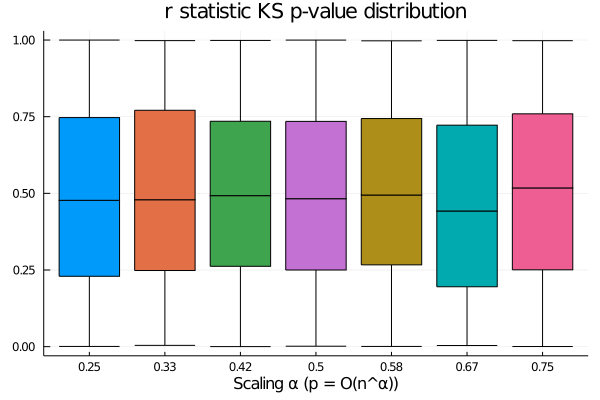
\includegraphics[scale=0.5]{r}
    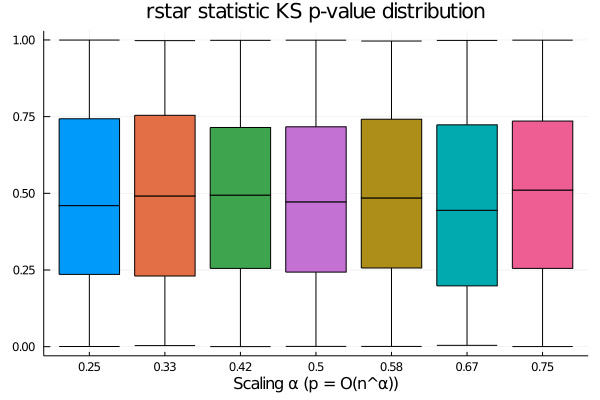
\includegraphics[scale=0.5]{rstar}
    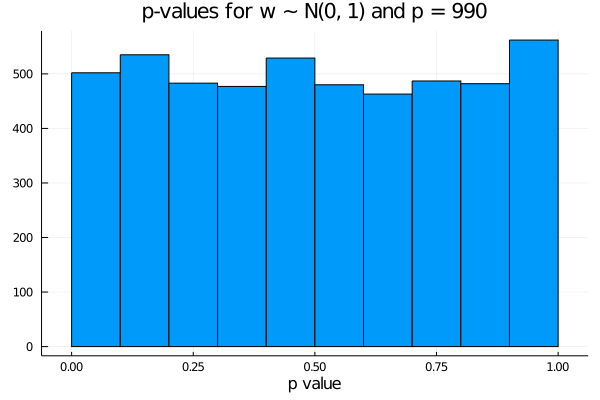
\includegraphics[scale=0.5]{w_largep}
\end{figure}

\newpage


\subsection{Multivariate normal distribution as an exponential family}
To benefit from the many existing results concerning exponential families, we reformulate the density (\ref{eq-density-omega}) as an exponential family with sufficient statistic $T$ and natural parameter $\theta \in \text{vec}(\mathcal{S}_p)$. 
\begin{equation} \label{eq-density-theta}
    f(x; \theta) = \exp\left(\theta^\top T(x) + \frac{1}{2}\log\left(|\text{mat}(\theta)|\right) - \frac{p}{2}\log\left(2\pi\right)\right),
\end{equation}
where the sufficient statistic $T : \mathbb{R}^p \rightarrow \mathcal{S}_p$ is given by $T(x) = \text{vec}(xx^t)$. Note that the canonical parameter $\theta$ is simply the vector reprensentation of the precision matrix of the multivariate normal distribution. For convenience, we use $\Omega(\theta) = (\omega_{i,j}(\theta))_{i,j}$ and $\Sigma(\theta) = (\sigma_{i,j}(\theta))_{i,j}$ to be the precision matrix and correlation matrix corresponding to the natural parameter $\theta$.

\subsection{Cumulants of the multivariate normal distributrion}

We are now interested in computing the first and second order cumulants of the multivariate normal distribution. In an exponential family with canonical parameter $\theta$ and sufficient statistic $T$, the first and second order cumulants $\kappa_i, \kappa_{i, j}$ are given by
\begin{align*}
    \kappa_i(\theta) = \mathbb{E}_\theta\left[T_i(X)\right] && \kappa_{i,j}(\theta) = \text{Cov}_\theta\left[T_i(X), T_j(X)\right].
\end{align*}

Starting with the first order cumulants, let $i \in [p(p+1)/2]$ the sufficient statistic $T$ at index $i$ is equal to $T_i(x) = x_kx_l$ for some $k \leq l$, hence
\begin{equation*}
    \kappa_i(\theta) 
    = \mathbb{E}_\theta\left[T_i(X)\right]
    = \mathbb{E}_\theta\left[X_kX_l  \right]
    = \left\{
        \begin{array}{cc}
            \text{Var}_\theta[X_k]      & \text{ if } k = l,\\
            \text{Cov}_\theta[X_k, X_l] & \text{ if } k \neq l
        \end{array}
    \right\}
    = \sigma_{k, l}(\theta).
\end{equation*}

For the second order cumulants, let $i, j \in [p(p+1)/2]$ with $T_i(x) = x_kx_l$ and $T_j(x) = x_mx_n$ for some $k \leq l$ and $m \leq n$, we then have
\begin{align*}
    \kappa_{i,j}(\theta)
    &= \text{Cov}_\theta\left[T_i(X), T_j(X)\right]\\
    &= \mathbb{E}_\theta\left[T_i(X)T_j(X)\right] - \mathbb{E}_\theta\left[T_i(X)\right]\mathbb{E}_\theta\left[T_j(X)\right]\\
    &= \mathbb{E}_\theta\left[X_kX_lX_mX_n\right] - \sigma_{k, l}(\theta)\sigma_{m, n}(\theta).
\end{align*}
By Isserlis' theorem \cite{Isserlis1918}, the fourth moment term $\mathbb{E}_\theta\left[X_kX_lX_mX_n\right]$ is
\begin{equation*}
    \mathbb{E}_\theta\left[X_kX_lX_mX_n\right] = \sigma_{k,l}(\theta)\sigma_{m,n}(\theta) + \sigma_{k,m}(\theta)\sigma_{l,n}(\theta) + \sigma_{k,n}(\theta)\sigma_{l,m}(\theta),
\end{equation*}
giving the following expressing for the second order cumulant $\kappa_{i,j}(\theta)$
\begin{equation*}
    \kappa_{i,j}(\theta) = \sigma_{k,m}(\theta)\sigma_{l,n}(\theta) + \sigma_{k,n}(\theta)\sigma_{l,m}(\theta).
\end{equation*}

% \section{Exponential families facts}

\begin{itemize}
    \item $ f_X(x; \gamma) = h(x)\exp\left(\gamma^\top T(x) - A(\gamma) \right) $
    \item $ A(\gamma) = \log \int h(x)\exp\left(\gamma^\top T(x)\right) \d x $
    \item $A'(\gamma) = \mathbb{E}_\gamma[T(X)]$
    \item $\ell(\theta) = \gamma^\top T(x) - A(\gamma) \Rightarrow \ell'(\theta) = T(x) - A'(\gamma) \Rightarrow A'(\hat\gamma) = T(x)$
    \item $A'(\hat\gamma) = T(x)$ and $A'(\gamma) = \mathbb{E}_\gamma[T(X)] \Rightarrow \mathbb{E}_{\hat\gamma}[T(X)] = T(x)$
    \item $f_X(x; \gamma) = h(x)\exp\left(\gamma^\top T(x) - A(\gamma) \right) = h(x)\exp\left(\gamma^\top A'(\hat\gamma) - A(\gamma) \right) = h(x)g_\gamma(\hat\gamma) \Rightarrow \hat\gamma$ is sufficient by Fisher-Neyman
    \item $T(X) = X \Rightarrow \mathcal{K}_X(t \mid \gamma) = \log \mathbb{E}_\gamma[\exp(t^\top X)] = A(\gamma + t) - A(\gamma) $
    \item $T(X) = X \Rightarrow \nabla_t \mathcal{K}_X(t \mid \gamma) = \mathbb{E}_{\gamma + t}[X] $
    \item $T(X) = X \Rightarrow \hat\gamma = \nabla_t \mathcal{K}_X(t) |_{t=0}$
\end{itemize}



% \section{Assumptions}

% \section{Questions}

% \subsection{What is $p^*$?}

% \subsection{Convergence $p^* \rightarrow p$}

% \subsection{Is $p^* \rightarrow p$ true in high dimensions?}

% \subsection{What is $r^*$?}

% \subsection{Asymptotic normality of $r^*$}

% \subsection{Is $r^*$ asymptotically normal in high dimensions?}

% \subsection{What are Gaussian Graphical Models (GGM)?}

\bibliographystyle{plain}
\bibliography{references}

\nocite{*}

\end{document}
